% @Author: Athul Vijayan
% @Date:   2014-09-03 14:16:33
% @Last Modified by:   Athul Vijayan
% @Last Modified time: 2014-09-04 22:58:22

\documentclass[11pt,paper=a4,answers]{exam}
\usepackage{graphicx,lastpage}
\usepackage{upgreek}
\usepackage{censor}
\usepackage{amsmath}
\usepackage{enumerate}
\censorruledepth=-.2ex
\censorruleheight=.1ex
\hyphenpenalty 10000
\usepackage[paperheight=10.5in,paperwidth=8.27in,bindingoffset=0in,left=0.8in,right=1in,
top=0.7in,bottom=1in,headsep=.5\baselineskip]{geometry}
\flushbottom
\usepackage[normalem]{ulem}
\renewcommand\ULthickness{2pt}   %%---> For changing thickness of underline
\setlength\ULdepth{1.5ex}%\maxdimen ---> For changing depth of underline
\renewcommand{\baselinestretch}{1}
\pagestyle{empty}

\pagestyle{headandfoot}
\headrule
\newcommand{\continuedmessage}{%
\ifcontinuation{\footnotesize Question \ContinuedQuestion\ continues\ldots}{}%
 }
\runningheader{\footnotesize CH5440}
{\footnotesize Applied Time series}
{\footnotesize Page \thepage\ of \numpages}
\footrule
\footer{\footnotesize}
{}
{\ifincomplete{\footnotesize Question \IncompleteQuestion\ continues
on the next page\ldots}{\iflastpage{\footnotesize End of Assignment}{\footnotesize Please go        on to the next page\ldots}}}

\usepackage{cleveref}
\crefname{figure}{figure}{figures}
\crefname{question}{question}{questions}
%==============================================================
\begin{document}

%% \thispagestyle{empty}

\noindent
\begin{minipage}[l]{.1\textwidth}%
\noindent
% \includegraphics[width=1.5\textwidth]{123}
\end{minipage}
\hfill
\begin{minipage}[r]{.68\textwidth}%
\begin{center}
{\large \bfseries IIT Madras \par
\Large Applied Time Series \\[2pt]
\small Assignment 2  \par}
%  \vspace{0.5cm}
\end{center}
\end{minipage}
\fbox{\begin{minipage}[l]{.195\textwidth}%
\noindent
{\footnotesize \today}
\end{minipage}}
\par
\noindent
\uline{ED11B004   \hfill \normalsize\emph \hfill       Athul Vijayan}
\begin{questions}

\pointformat{\boldmath\themarginpoints}
\question
\begin{enumerate}[(a)]
\item
We have $x[k] = \phi_1 x[k-1] + e[k]$ where $e[k] \sim \mathcal{N}(0, \sigma_e ^2)$ and $|\phi_1| < 1$.
\begin{align}
    cov(x[k], x[k-l]) &= E(x[k] \quad x[k-l]) \nonumber \\
    &= E((\phi_1 x[k-1] + e[k]) \quad x[k-l]) \nonumber \\
    &= \phi_1 E(x[k-1] x[k-l]) + E(e[k] x[k-l]) \nonumber\\
    &= \phi_1 ^2 E(x[k-2] x[k-l])  \nonumber\\
    \vdots \nonumber \\
    &= \phi_1 ^l var(x[k-l])
\end{align}
Now:
\begin{align}
    corr(x[k], x[k-l]) &= \frac{cov(x[k], x[k-l])}{\sqrt{var(x[k])var(x[k-l])}} \nonumber \\
    &= \phi_1 ^l \left[ \frac{var(x[k-l])}{var(x[k])}\right]^{1/2} \nonumber
\end{align}
\item 
For AR(1) process $x[k] = \phi_1 x[k-1] + e[k]$ where $e[k] \sim \mathcal{N}(0, \sigma_e ^2)$ and $|\phi_1| < 1$,

\begin{align}
    x[k] &= \phi_1 x[k-1] + e[k] \nonumber \\
    &= \phi_1^2 x[k-2] + \phi_1 e[k-1] + e[k] \nonumber \\
    &= \phi_1^2 x[k-2] + \phi_1 e[k-1] + e[k] \nonumber \\
    \vdots \nonumber \\
    \text{making $l$ backward recursions} \nonumber\\
    x[k] &= \phi_1 ^l x[k-l] + \sum_{i=0}^{l-1} \phi_1 ^i e[k-i]
\end{align}
We can rewrite it as:
$$
x[k] - \sum_{i=0}^{l-1} \phi_1 ^i e[k-i] =  \phi_1 ^l x[k-l]  \nonumber \\
$$
Now consider the RHS as l goes to $\infty$. i.e for large times.\\
$$
\lim_{l \to \infty} \phi_1 ^l x[k-l] = 0 \qquad \text{Since $|\phi_1| < 1$}
$$
Which gives us:\\
\begin{align}
    x[k] = \sum_{i=0}^{\infty} \phi_1 ^i e[k-i]
\end{align}
\item To prove stationarity, we will show $corr(x[k], x[k-l])$ is a function of $l$ at large times.\\
\begin{align}
    cov(x[k], x[k-l]) = E\left[ \left(\sum_{i=0}^{\infty} \phi_1 ^i e[k-i] \right) \left(\sum_{i=0}^{\infty} \phi_1 ^i e[k-l-i] \right)\right] \nonumber \\
    = E\left[(e[k] + \phi_1 e[k-1] + \phi_1 ^2 e[k-2] + \cdots) (e[k-l] + \phi_1 e[k-l-1] + \phi_1 ^2 e[k-l-2] + \cdots) \right] \nonumber
\end{align}
\begin{align}
    cov(x[k], x[k-l]) &= \sigma_e ^2 \sum_{k=0}^{\infty} \phi_1^{l+k} \phi_1^{k} \nonumber \\
    &= \phi_1 ^l \sigma_e ^2 \sum_{k=0}^{\infty} \phi_1^{2k} \nonumber \\
    \sigma_{xx}[l] &= \frac{\phi_1 ^l \sigma_e ^2}{1-\phi_1 ^2} \qquad \text{for } l \geq 0 \nonumber\\
    \rho_{xx}[l] &= \frac{\sigma_{xx}[l]}{\sigma_{xx}[0]} \nonumber \\
    \rho_{xx}[l] &= \phi_1 ^l \nonumber
\end{align}
This proves that $corr(x[k], x[k-l])$ is a function of lag $l$ only and not the particulat sample itself. thus stationary for large times.\\
\item in equation (2), if we make k backward recursions to reveal $x[0]$, \\
$$
x[k] = \phi_1 ^k x[0] + \sum_{i=0}^{k-1} \phi_1 ^i e[k-i]
$$
For it to be stationary, first term should vanish. i.e. $x[0] = 0$.
\end{enumerate}
\question
We have MA(2) process as $\qquad v[k] = e[k] + c_1 e[k-1] + c_2 e[k-2]$
\begin{enumerate}[(a)]
    \item 
    $$
    H(q^{-1}) = 1 + c_1 q^{-1} + c_2 q^{-2}
    $$
    We have ACVF generating function:\\
    \begin{align}
        g_\sigma(z) &= \sigma_e ^2 H(z^{-1}) H(z) \nonumber \\
        &= (1 + c_1 z^{-1} + c_2 z^{-2}) (1 + c_1 z + c_2 z^2) \sigma_e \nonumber \\
        &= (1 + c_1 ^2 + c_2 ^2 + z(c_1 + c_1 c_2) + z^{-1} (c_1 + c_1 c_2) + z^{-2} c_2 + z^2 c_2) \sigma_e \nonumber
    \end{align}
    Comparing this with definition of ACF generating function:
    $$
    g_\sigma (z) = \sum_{l=-\infty}^{+\infty} \sigma_{vv}[l] z^{-l}
    $$
    comparing coefficients of $z$ and $z^{-1}$ :\\
    $$
    \sigma_{xx}[l] = \begin{cases}
        (1 + c_1 ^2 + c_2 ^2)\sigma_e ^2  & \qquad \text{when $l = 0$}\\
        (c_1 + c_1 c_2) \sigma_e ^2  & \qquad \text{when $|l| = 1$}\\
        c_2 \sigma_e ^2  & \qquad \text{when $|l| = 2$}\\
        0  & \qquad \text{when $|l| > 2$}\\
        \end{cases}
    $$
    \item For invertibility (and in turn stability) can be achieved by having roots of $H(z^{-1})$ reside outside unit circle.\\
    \begin{align}
        1 + c_1 z^{-1} + c_2 z^{-2} = 0 \nonumber\\
        z^{-1} = \frac{-c_1 \pm \sqrt{c_1^2 - 4c_2}}{2 c_2} > 1  \nonumber
    \end{align}
    \item
    For an AR(2) process :$$ H(q^{-1})v[k] = e[k]$$
    where $H(q^{-1}) = 1 - 1.3q^{-1} + 0.4q^{-2}$\\
    We have
    \begin{align}
        x[k] &= 1.3x[k-1] - 0.4x[k-2] + e[k] \nonumber \\
        x[k]x[k-1] &= 1.3x[k-1]x[k-1] - 0.4x[k-2]x[k-1] + e[k]x[k-1] \nonumber \\
        x[k]x[k-2] &= 1.3x[k-1]x[k-2] - 0.4x[k-2]x[k-2] + e[k]x[k-2] \nonumber \\
        \vdots &= \vdots \nonumber
    \end{align}
    taking expectation and dividing by $\sigma[0]$ gives general difference equation for ACF
    \begin{align}
        \rho[k] = 1.3\rho[k-1] - 0.4\rho[k-2] \nonumber
    \end{align}
\end{enumerate}
\question
We have $\qquad y[k] = Asin(2\pi f_0 k) + e[k]$\\
\begin{enumerate}[(a)]
    \item To prove not stationary, we consider $E(y[k])$ \\
    \begin{align}
        E(y[k]) &= E(Asin(2\pi f_0 k) + e[k]) \nonumber \\
        &= A.E(sin(2\pi f_0 k)) \nonumber
    \end{align}
    whick is a function of k. i.e. its dependent on the sample point. so not stationary.
    \item
    to be done
    \item Since $y[k]$ is affected by the white noise term, we may not be even able to see the periodicity in $y[k]$ depending on the variance or noise part. But if there is a periodic signal in $y[k]$, it will be evident in ACF of $y[k]$ since there is no noise term. It  will be just a sinusoidal term.\\
    So it will be much easier to say periodicity from ACF than $y[k]$.
\end{enumerate}
\question
\begin{enumerate}[(a)]
    \item \begin{enumerate}[(i)]
        \item $$x_1 [k] - 0.7x[k - 1] + 0.12x[k - 2] = e[k]$$
        at lag $l = 1$, PACF is same as ACF since no intermediate term to condition.\\
        $\longrightarrow$ ACF of AR(2) process for lag $=1$.\\
        $$\sigma [1] - 0.7 \sigma[0] + 0.12 \sigma [1] = 0$$
        $$\rho [1]  =\frac{0.7}{1+0.12} = 0.625$$
        at lag $l=2$, we need to condition both $x[k]$ and $x[k-2]$ from $x[k-1]$.\\
        conditioned $x[k]$ is represented as $\eta [k] = x[k] - \hat{x} [k]$ where $\hat{x} [k] = \alpha x[k-1]$ where optimal $\alpha = \rho[1]$. similarly $\eta [k-2]$.\\
        Now we have:
        \begin{align}
            \phi [2] &= corr(\eta [k], \eta [k-2]) \nonumber \\
            &= corr(x[k] - 0.625 x[k-1], x[k-2] - 0.625 x[k-1]) \nonumber \\
            &= \rho[2] - 1.25 \rho[1] + 0.390625 \rho[0] \nonumber \\
            &= -0.073125 \qquad ; \rho[2] = 0.3175 \nonumber
        \end{align}
        And using R: $\phi [1] = 0.625$  and $\phi [2] = -0.120$\\
        \item
        $$x_2 [k] = e[k] + 0.4e[k-1]$$
        similar to above, $\phi[1] = \rho[1] = \frac{0.4}{1+.4^2} = 0.3448$\\
        \begin{align}
            \phi[2] &= corr(\eta [k], \eta [k-2]) \nonumber \\
            &= corr(x[k] - 0.3448 x[k-1], x[k-2] - 0.3448 x[k-1])\\
            &= \rho[2] - 0.6896\rho[1] + 0.118887 \rho[0] \nonumber \\
            &= -0.1189741 \qquad ; \rho[2] = 0 \nonumber
        \end{align}
        And using R: $\phi [1] = 0.3448276$  and $\phi [2] = -0.1349528$\\
    \end{enumerate}
    \item \begin{enumerate}
        \item EuStockMarkets (SMI)\\
        Data:\\
        \centerline{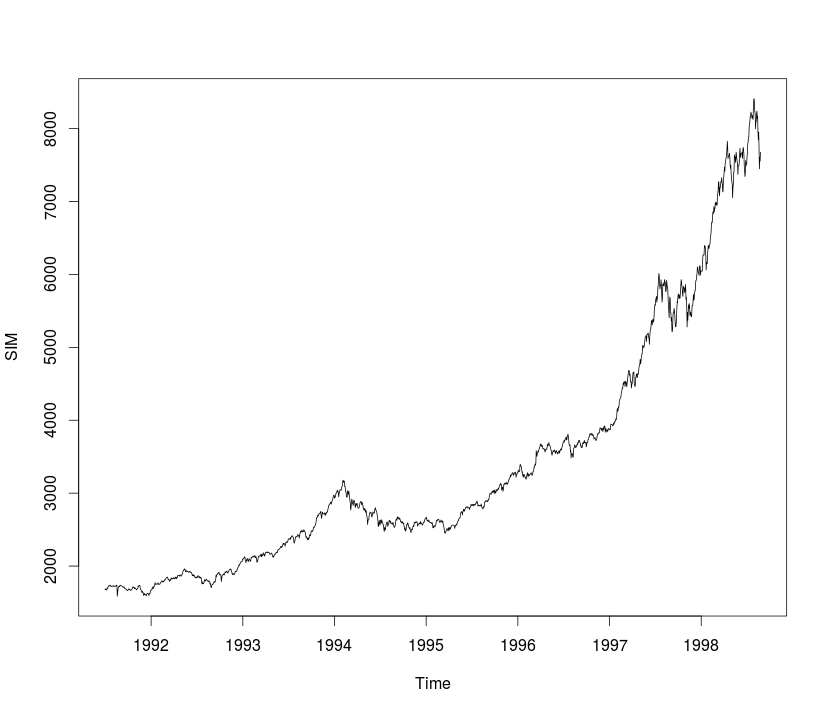
\includegraphics[width=6cm]{sim.png}}
        \newpage
        ACF:\\
        \centerline{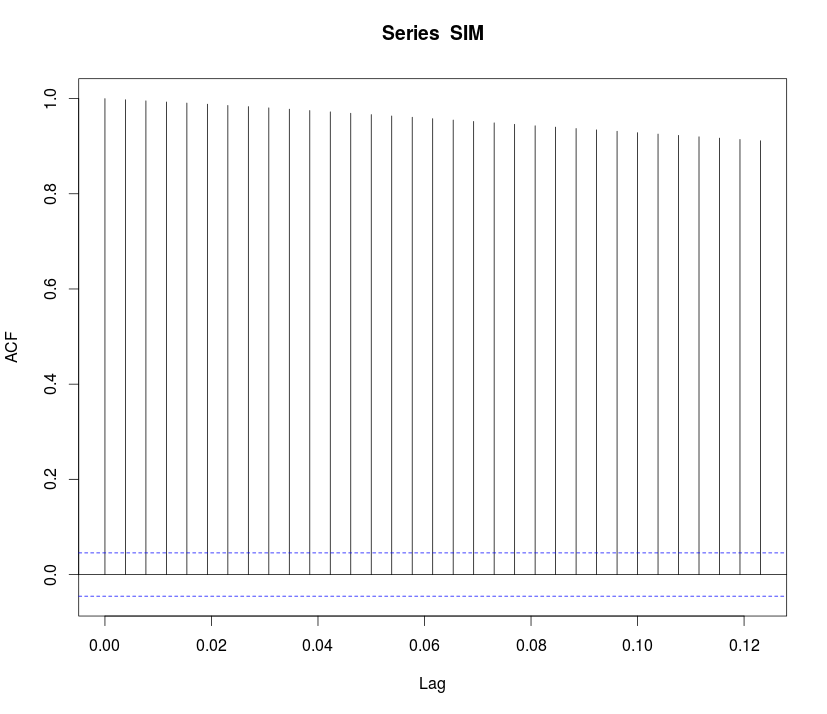
\includegraphics[width=6cm]{simacf.png}}
        PACF:\\
        \centerline{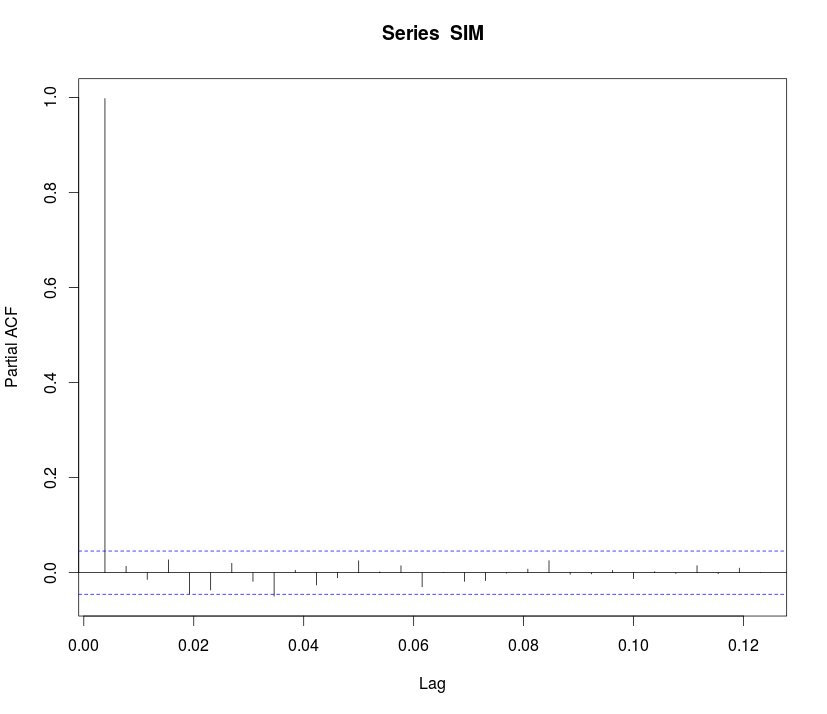
\includegraphics[width=6cm]{simpacf.png}}
        The process is non-periodic. From PACF we can see its an AR(1) process. ACF is dying very slow, could be because $d$ is nearly equal to one.

        \item Nottem\\
        Data:\\
        \centerline{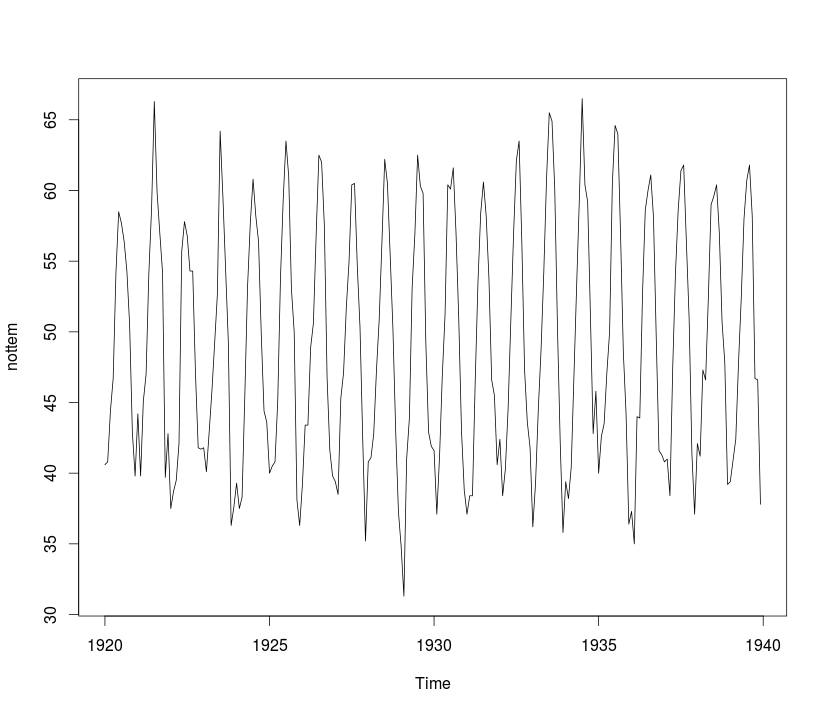
\includegraphics[width=6cm]{not.png}}
        \newpage
        ACF:\\
        \centerline{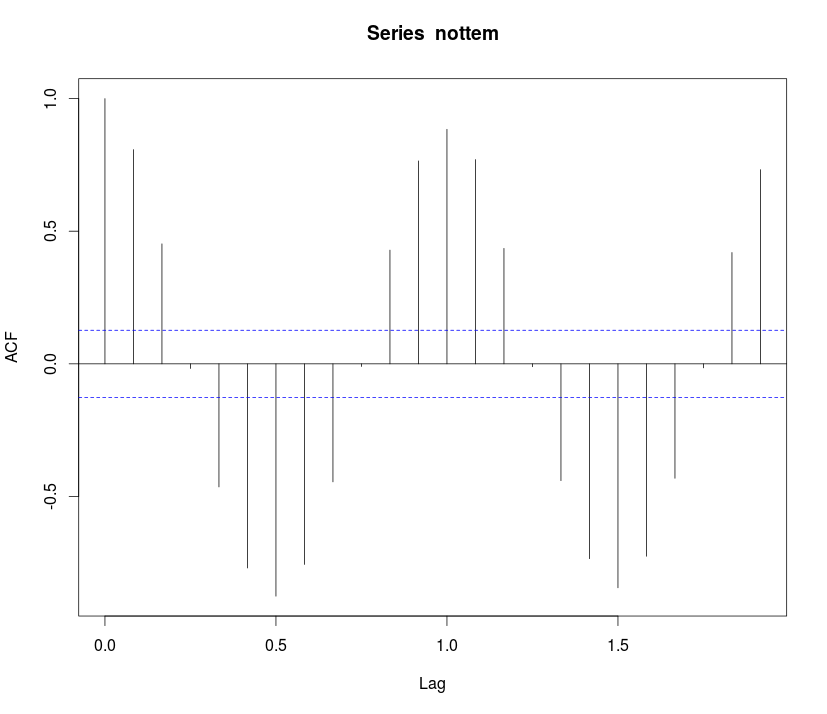
\includegraphics[width=6cm]{nacf.png}}
        PACF:\\
        \centerline{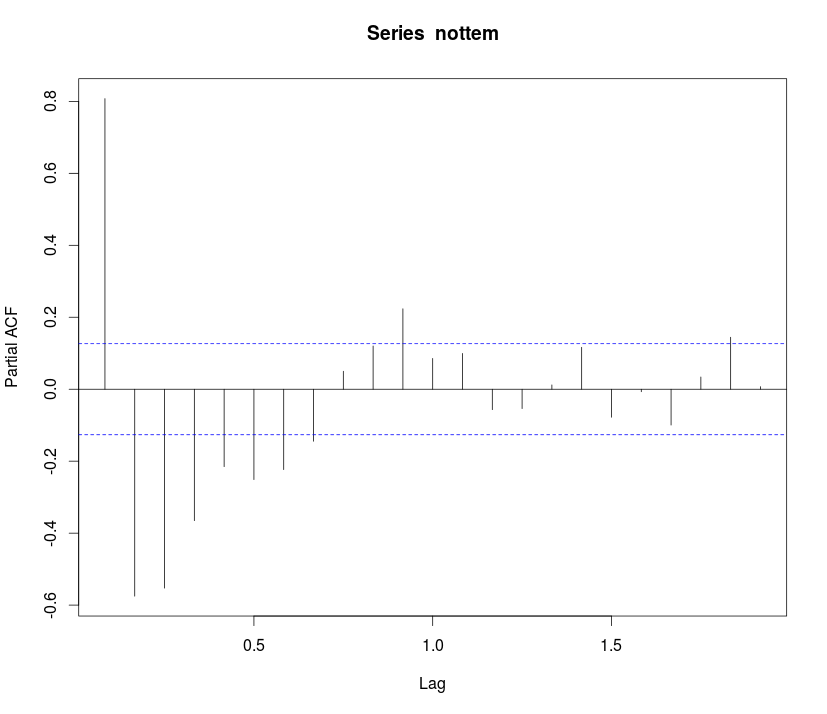
\includegraphics[width=6cm]{npacf.png}}
        This is periodic and has a sinusoidal signal in it. The sinusoidal element can be confirmed by the sinusoidal nature of ACF.
    \end{enumerate}
\end{enumerate}
\question
To be done in R.
\end{questions}
\begin{center}
\rule{.7\textwidth}{1pt}
\end{center}
\end{document} 